%!TEX program = pdflatex
% Full chain: pdflatex -> bibtex -> pdflatex -> pdflatex
\documentclass[11pt,en]{elegantpaper}

\title{ElegantPaper: An Elegant \LaTeX{} Template for Working Papers}
\author{\href{https://ddswhu.me/}{Dongsheng Deng}}
\institute{\href{https://github.com/ElegantLaTeX}{Elegant\LaTeX{} Program}}
\version{0.07}
\date{\today}


\begin{document}

\maketitle

\begin{abstract}
This paper illustrates the usage of the \href{https://github.com/ElegantLaTeX/ElegantPaper}{ElegantPaper} template, which is designed for writing a working paper. This template is based on the standard \LaTeX{} article class. The goal of this template is to make the writing process easier and more comfortable. You can get rid of all the worries about the format. Just enjoy it! If you have any questions, suggestions or bug reports, you can visit \href{https://github.com/ElegantLaTeX/ElegantPaper/issues}{ElegantPaper/issues}. Looking for other templates designed by Elegant\LaTeX{} Group? Please visit: \href{https://github.com/ElegantLaTeX}{https://github.com/ElegantLaTeX}.\par
\keywords{Elegant\LaTeX{}, Working Paper, Template}
\end{abstract}


\section{Introduction}

This template is based on the standard \LaTeX{} article class, which means you can pass the arguments of article class to it (\lstinline{a4paper}, \lstinline{10pt} and etc.)( \lstinline{11pt} is recommended). It supports different engines, You can choose either \lstinline{PDFLaTeX} or \lstinline{XeLaTeX}\footnote{with \lstinline{ctex} package for Chinese fonts settings.}.  

The effect of math fonts is as follows:
\begin{equation}
(a+3b)^{n} = \sum_{k=0}^{n} C_{n}^{k} a^{n-k} (3b)^k  \label{eq:binom}
\end{equation}

\subsection{Global Options}
I defined one option named \lstinline{lang}, this option has two alternative values, \lstinline{lang=en} (default) or \lstinline{lang=cn}. \lstinline{lang=cn} will make the caption of figure/table, abstract name, refname etc. Chinese, while \lstinline{lang=en} will keep all these stuff English, as the default article class sets. You can use this option as
\begin{lstlisting}
\documentclass[lang=en]{elegantpaper}
\documentclass{en}{elegantpaper} % both ok
\end{lstlisting}

\subsection{Custom Commands}

I didn't change any default command or environment, which means you can use all the basic \LaTeX{} commands and environments as before.  Besides, I defined 4 commands
\begin{enumerate}
	\item \lstinline{\email}: create the hyperlink to email address.
	\item \lstinline{\figref}: same usage as \lstinline{\ref}, but start with label text <\textbf{Figure n}>.
	\item \lstinline{\tabref}: same usage as \lstinline{\ref}, but start with label text <\textbf{Table n}>.
	\item \lstinline{\keywords}: create the keywords in the abstract section.
\end{enumerate}{}

\subsection{List Environments}
You can use \lstinline{itemize}, \lstinline{enumerate}, or \lstinline{description} environment as below\\
\begin{minipage}[c]{0.51\linewidth}
\begin{lstlisting}
\begin{itemize}
    \item Routing and resource discovery;
    \item Resilient and scalable networks;
    \item Distributed storage and search.
\end{itemize}
\end{lstlisting}
\end{minipage}
\begin{minipage}[c]{0.48\linewidth}
\begin{itemize}
    \item Routing and resource discovery;
    \item Resilient and scalable networks;
    \item Distributed storage and search.
\end{itemize}
\end{minipage}

\subsection{Table}
I strongly recommend you to use the \lstinline{booktabs} package in your paper. It adds three commands to make the table prettier,  \lstinline{\toprule}, \lstinline{\midrule} and \lstinline{\bottomrule}. \tabref{tab:reg} is an example.
\begin{lstlisting}
\begin{table}[htbp]
  \small
  \centering
  \caption{Auto MPG and Price \label{tab:reg}}
    \begin{tabular}{lcc}
    \toprule
                    &       (1)         &        (2)      \\
    \midrule
    mpg             &    -238.90***     &      -49.51     \\
                    &     (53.08)       &      (86.16)    \\
    weight          &                   &      1.75***    \\
                    &                   &      (0.641)    \\
    constant        &     11,253***     &       1,946     \\
                    &     (1,171)       &      (3,597)    \\
    obs             &        74         &         74      \\
    $R^2$           &      0.220        &       0.293     \\
    \bottomrule
    \multicolumn{3}{l}{\scriptsize Standard errors in parentheses} \\
    \multicolumn{3}{l}{\scriptsize *** p<0.01, ** p<0.05, * p<0.1} \\
    \end{tabular}%
\end{table}%
\end{lstlisting}
\begin{table}[htbp]
  \small
  \centering
  \caption{Auto MPG and Price \label{tab:reg}}
    \begin{tabular}{lcc}
    \toprule
                    &       (1)         &        (2)      \\
    \midrule
    mpg             &    -238.90***     &      -49.51     \\
                    &     (53.08)       &      (86.16)    \\
    weight          &                   &      1.75***    \\
                    &                   &      (0.641)    \\
    constant        &     11,253***     &       1,946     \\
                    &     (1,171)       &      (3,597)   \\
    obs             &        74         &         74     \\
    $R^2$           &      0.220        &       0.293    \\
    \bottomrule
    \multicolumn{3}{l}{\scriptsize Standard errors in parentheses} \\
    \multicolumn{3}{l}{\scriptsize *** p<0.01, ** p<0.05, * p<0.1} \\
    \end{tabular}%
\end{table}%



\subsection{Graphics}
To include a graphic, you can use figure environment as usual. \figref{fig:scatter} shows the effect. You can put all your images in the sub directories (\lstinline{./image/}, \lstinline{./img/}, \lstinline{./figure/}, \lstinline{./fig/}) of your current working directory.
\begin{lstlisting}
\begin{figure}[htbp]
	\centering
	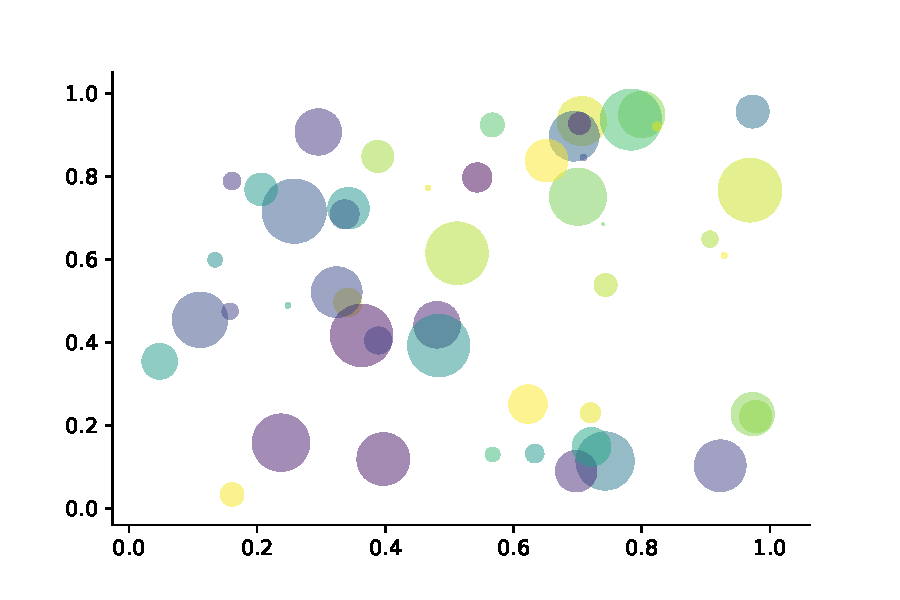
\includegraphics[width=0.6\textwidth]{scatter.pdf}
	\caption{Scatter Plot Example \label{fig:scatter}}
\end{figure}
\end{lstlisting}
\begin{figure}[htbp]
	\centering
	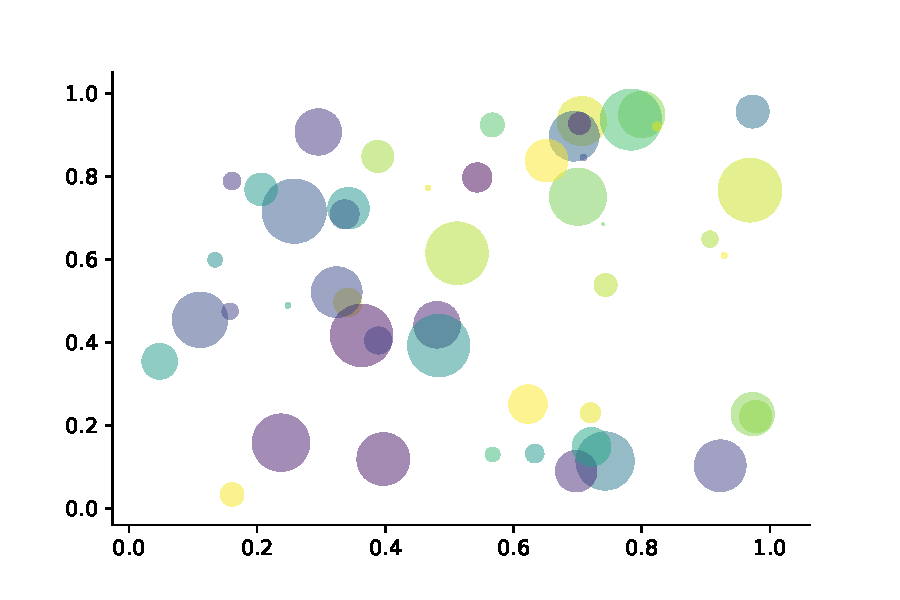
\includegraphics[width=0.6\textwidth]{scatter.pdf}
	\caption{Scatter Plot Example \label{fig:scatter}}
\end{figure}

\subsection{Bibliography}
This template used Bib\TeX{} to generate the bibliography, the default bibliography style is \lstinline{aer}. Let's take a glance at the citation effect, ~\cite{en3} used data from a major peer-to-peer lending marketplace in China to study whether female and male investors evaluate loan performance differently. 

If you want to use Bib\TeX{}, you must create a file named \lstinline{wpref.bib}, and add bib items (from Google Scholar, Mendeley, EndNote, and etc.) to \lstinline{wpref.bib} file, and cite the bibkey in the \lstinline{tex} file. The Bib\TeX{} will automatically generate the bibliography for you for the reference you cited. If you want to add some noncited references or all of them to the bibliography,  you can use 
\begin{lstlisting}
\nocite{EINAV2010, Havrylchyk2018} % add two noncited references 
\nocite{*} % list all the references of the bib file.
\end{lstlisting}



\section{A Minimal Example}
In this section, we give a simple example using this template.
\begin{lstlisting}
\documentclass[lang=en]{elegantpaper}

% title information
\title{A Working Paper Example}
\author{ddswhu} 
\institute{Elegant\LaTeX{} Group}
\version{1.00}
\date{\today}

\begin{document}

\maketitle

\begin{abstract}
Your abstract goes here.
\keywords{keyword1, keyword2}
\end{abstract}

\section{Introduction}
The content of introduction section.

\section{Conclusion}
The content of conclusion section.

% include the noncited reference
\nocite{ref1, ref2}
\bibliography{wpref}
\end{document}
\end{lstlisting}

\nocite{en1,en2}

\bibliography{wpref}

\end{document}
